\documentclass[a4paper]{report}

\usepackage{mythesis}

% Graphics directory
\graphicspath{{img/}}

% Title page options
\title{\thesisTitle{}}
\author{\studentName{}}
\date{\thesisDate{}}

% Bibliography
\bibliography{thesis}

%%%%%%%%%%%%%%%%%%%%%%%%%%%%%%%%%%%%%%%%%%%%%%%%%%%%%%%%%%%%%%%%%%%%%%%%%%%%%%%%

\begin{document}

%%%%%%%%%%%%%%%%%%%%%%%%%%%%%%%%%%%%%%%%%%%%%%%%%
% Title Page
%%%%%%%%%%%%%%%%%%%%%%%%%%%%%%%%%%%%%%%%%%%%%%%%%
\begin{titlepage}
\begin{center}

% Upper part of the page

\includegraphics[width=0.25\textwidth]{sydney_uni_coat_of_arms}\\[1cm]

\textsc{\LARGE \universityName{}}\\[1.5cm]

\textsc{\Large Final year thesis}\\[0.5cm]

% Title
\HRule \\[0.4cm]
{\huge \bfseries \thesisTitle{}}\\[0.4cm]
\HRule \\[1.5cm]

% Author and supervisor
\begin{minipage}{0.4\textwidth}
    \begin{flushleft} \large
        \emph{Author:}\\
        \studentName{}
    \end{flushleft}
\end{minipage}
\begin{minipage}{0.4\textwidth}
    \begin{flushright} \large
        \emph{Supervisor:} \\
        \supervisorName{}
    \end{flushright}
\end{minipage}

% strech vertical space so that it fills all empty space
\vfill

% Thesis description
{\large A thesis submitted in fulfilment of the requirements for the\\
degree of Bachelor of Engineering (Computer) in the \\
School of Electrical Engineering at\\
The University of Sydney}

% strech vertical space so that it fills all empty space
\vfill

% Bottom of the page
{\large \thesisDate{}}

\end{center}
\end{titlepage}

\pagenumbering{roman}

%%%%%%%%%%%%%%%%%%%%%%%%%%%%%%%%%%%%%%%%%%%%%%%%%
% Acknowledgements
%%%%%%%%%%%%%%%%%%%%%%%%%%%%%%%%%%%%%%%%%%%%%%%%%
\chapter*{Acknowledgements}
This project could not be completed without the guidance of my project 
supervisor, \supervisorName{}. He always made himself available to assist me 
with the understanding with many new and unknown concepts. His expertise in the 
field was a great asset and greatly contributed to my own understanding of the 
ideas explored in this thesis. His support and guidance was invaluable, and were
instrumental to the success of my project. 

Additionally, much of the works completed during this project could not have 
been performed without the prior research of \contributorOne{} and 
\contributorTwo{}. Both were generous enough to lend their own support and 
expertise in order to gain an understanding of the implemented random projection
algorithms.

%%%%%%%%%%%%%%%%%%%%%%%%%%%%%%%%%%%%%%%%%%%%%%%%%
%  Publications
%%%%%%%%%%%%%%%%%%%%%%%%%%%%%%%%%%%%%%%%%%%%%%%%%
\chapter*{Publications}
This thesis is based on the following publications:
\begin{enumerate}
\item \fullcite{Vries:2010}
\item \fullcite{Khoa:2012}
\item \fullcite{Bay:2003}
\end{enumerate}

%%%%%%%%%%%%%%%%%%%%%%%%%%%%%%%%%%%%%%%%%%%%%%%%%
% Abstract
%%%%%%%%%%%%%%%%%%%%%%%%%%%%%%%%%%%%%%%%%%%%%%%%%
\begin{abstract}
The prediction of the stock market has become an issue of great interest in the
fields of finance, mathematics and engineering; due mainly to its great 
potential financial gain. Many researchers have devised various algorithms and
differing approaches to the problem of stock market analysis, with varying 
degrees of success.

A major outstanding issue for stock market analysis is the effective and 
efficient detection of local anomalies in the input data sets, which are 
inherently highly multidimensional. Many na\"{\i}ve algorithms are highly 
inefficient and others fail to adequately detect the local anomalies altogether.
It had become a time-vs-correctness trade-off in which no accepted compromise
could be reached.

However, researchers are starting to explore the relatively new concept of 
applying ``random projections'' to the highly multidimensional data sets. 
Researchers have proven that by applying these random projections, they are
able to significantly reduce the dimensionality of the data sets, whilst 
sufficiently retaining the inherent properties of that data set --- at least so
much as anomaly detection is concerned.

Anomaly detection is important because it allows otherwise-accurate machine 
learning algorithms such as neural networks to more accurately model and 
predict the stock exchange data by ignoring anomaly data, which likely doesn't 
effect the state of the model to any significant degree.

\emph{Professor Sanjay Chawla} from the ``University of Sydney'' has in recent 
years conducted and supervised new and exciting research oriented around random 
projections. In particular, \emph{Nguyen Lu Dang Khoa}, under the supervision of
\emph{Professor Chawla} evaluated the use of traditional distance metrics, such
as Euclidean distance and Mahalanobis distance, in the application of local 
anomaly detection. Khoa proposed the use of the `commute time' metric, derived 
from random walks on graphs, in anomaly detection.
\end{abstract}

%%%%%%%%%%%%%%%%%%%%%%%%%%%%%%%%%%%%%%%%%%%%%%%%%
% Table of Contents
%%%%%%%%%%%%%%%%%%%%%%%%%%%%%%%%%%%%%%%%%%%%%%%%%
\tableofcontents

%%%%%%%%%%%%%%%%%%%%%%%%%%%%%%%%%%%%%%%%%%%%%%%%%
% List of Figures
%%%%%%%%%%%%%%%%%%%%%%%%%%%%%%%%%%%%%%%%%%%%%%%%%
\listoffigures

%%%%%%%%%%%%%%%%%%%%%%%%%%%%%%%%%%%%%%%%%%%%%%%%%
% List of Algorithms
%%%%%%%%%%%%%%%%%%%%%%%%%%%%%%%%%%%%%%%%%%%%%%%%%
\listofalgorithms

%%%%%%%%%%%%%%%%%%%%%%%%%%%%%%%%%%%%%%%%%%%%%%%%%
% List of Tables
%%%%%%%%%%%%%%%%%%%%%%%%%%%%%%%%%%%%%%%%%%%%%%%%%
\listoftables
\pagenumbering{arabic}

%%%%%%%%%%%%%%%%%%%%%%%%%%%%%%%%%%%%%%%%%%%%%%%%%
% CHAPTER 01: Introduction
%%%%%%%%%%%%%%%%%%%%%%%%%%%%%%%%%%%%%%%%%%%%%%%%%
\chapter{Introduction}
\label{ch:intro}

%%%%%%%%%%%%%%%%%%%%%%%%%%%%%%%%%%%%%%%%%%%%%%%%%
% Motivation
%%%%%%%%%%%%%%%%%%%%%%%%%%%%%%%%%%%%%%%%%%%%%%%%%
\section{Motivation}
\label{sec:motivation}
\input{ch01-motivation}

%%%%%%%%%%%%%%%%%%%%%%%%%%%%%%%%%%%%%%%%%%%%%%%%%
% Contributions of this thesis
%%%%%%%%%%%%%%%%%%%%%%%%%%%%%%%%%%%%%%%%%%%%%%%%%
\section{Contributions of this thesis}
\label{sec:contributions}
\input{ch01-contributions}

%%%%%%%%%%%%%%%%%%%%%%%%%%%%%%%%%%%%%%%%%%%%%%%%%
% Organization
%%%%%%%%%%%%%%%%%%%%%%%%%%%%%%%%%%%%%%%%%%%%%%%%%
\section{Organization}
\label{sec:organization}
The rest of this thesis is organized as follows. In \hyperref[ch:background]
{Chapter~\ref{ch:background}}, we provide background to various anomaly 
detection techniques, as well as randomization techniques. In order to provide 
the reader with an understanding of the background topics, a brief background is
given to various topics in linear algebra, vector calculus and graph theory. In
\hyperref[ch:reconfigurableComputing]{Chapter~\ref{ch:reconfigurableComputing}}, 
we provide an overview of reconfigurable computing, including an explanation of 
Field-Programmable Gate Arrays (FPGAs).

In \hyperref[ch:design] {Chapter~\ref{ch:design}}, we profile the execution of 
an anomaly detection algorithm and explore possible improvements to the 
algorithm, in particular by outsourcing various stages of the algorithm to an 
FPGA device. In \hyperref[ch:implementation]{Chapter~\ref{ch:implementation}}, 
we describe the implementation of the improved algorithm and detail the process 
that was followed in order to construct the hardware processing device. In 
\hyperref[ch:results]{Chapter~\ref{ch:results}}, we record results obtained by 
benchmarking the device that was previously designed and constructed, and 
comparing the expected improvements to the algorithm's execution with the 
measured results.

We conclude in \hyperref[ch:conclusions] {Chapter~\ref{ch:conclusions}} by 
reflecting upon the results obtained through this research, and making 
suggestions for further research in this topic.

 
%%%%%%%%%%%%%%%%%%%%%%%%%%%%%%%%%%%%%%%%%%%%%%%%%
% Schedule
%%%%%%%%%%%%%%%%%%%%%%%%%%%%%%%%%%%%%%%%%%%%%%%%%
\section{Schedule}
\label{sec:schedule}
A Gantt chart showing the anticipated schedule for the project is shown in 
\hyperref[fig:ganttChart]{Figure~\ref{fig:ganttChart}}. This will be updated as 
the project progresses.

% Gantt chart
% See http://www.martin-kumm.de/tex_gantt_package.php
\begin{figure}[h]
	\begin{center}
		\scalebox{0.5}{
		\begin{gantt}[
				xunitlength=0.5cm,
				fontsize=\small,
				titlefontsize=\small,
				drawledgerline=true
				]{18}{36}
			% Months
			\begin{ganttitle}
				\titleelement{Mar}{4}
				\titleelement{Apr}{4}
				\titleelement{May}{4}
				\titleelement{Jun}{4}
				\titleelement{Jul}{4}
				\titleelement{Aug}{4}
				\titleelement{Sep}{4}
				\titleelement{Oct}{4}
				\titleelement{Nov}{4}
			\end{ganttitle}
			% Split months into quarters
			\begin{ganttitle}
				\numtitle{1}{1}{4}{1}
				\numtitle{1}{1}{4}{1}
				\numtitle{1}{1}{4}{1}
				\numtitle{1}{1}{4}{1}
				\numtitle{1}{1}{4}{1}
				\numtitle{1}{1}{4}{1}
				\numtitle{1}{1}{4}{1}
				\numtitle{1}{1}{4}{1}
				\numtitle{1}{1}{4}{1}
			\end{ganttitle}

			% Tasks
			\ganttbar{Background Reading}{1}{6}
			\ganttbar{Literature Review}{1}{24}
			
			\ganttbar{Performance Benchmarking}{7}{1} \ganttcon{7}{2}{7}{4}
			\ganttbarcon{Algorithm Analysis}{8}{1}				
			\ganttbarcon{MATLAB-to-C code transformation}{9}{2}
			\ganttbarcon{Code Improvements}{11}{4}			
			
			\ganttbarcon{Design of FPGA hardware}{15}{8}		
			
			\ganttbar{Implementation of FPGA hardware}{22}{4}
			\ganttbar{Testing and Debugging}{25}{2}			
			\ganttbar{Performance Benchmarking}{26}{2}
			
			\ganttbar{Review}{23}{8}
			
			% Milestones
			\ganttmilestone{Topic Proposal Due}{6.68} % April 20
			\ganttmilestonecon{Progress Report Due}{12} % June 1
			\ganttmilestonecon{Draft Treatise Due}{29.56} % October 12
			\ganttmilestonecon{Final Treatise Due}{31.08} % October 24
			\ganttmilestonecon{Project Presentations}{33.2} % November 9
		\end{gantt}
		}
	\end{center}
	\caption{Schedule for thesis work}
	\label{fig:ganttChart}
\end{figure}



%%%%%%%%%%%%%%%%%%%%%%%%%%%%%%%%%%%%%%%%%%%%%%%%%
% CHAPTER 02: Background
%%%%%%%%%%%%%%%%%%%%%%%%%%%%%%%%%%%%%%%%%%%%%%%%%
\chapter{Background}
\label{ch:background}

%%%%%%%%%%%%%%%%%%%%%%%%%%%%%%%%%%%%%%%%%%%%%%%%%
% ANOMALY DETECTION
%%%%%%%%%%%%%%%%%%%%%%%%%%%%%%%%%%%%%%%%%%%%%%%%%
\section{Anomaly detection}
\label{sec:anomalyDetection}
Anomaly detection is the process of detecting patterns in a given data set that 
do not conform to an established normal behavior \cite{Chandola:2007}.

The importance of anomaly detection is due to the fact that anomalies in data
translate to significant (and often critical) actionable information in a wide 
variety of application domains \cite{Chandola:2007}.

% WHAT ARE ANOMALIES?
\subsection{What are anomalies?}
\label{sec:whatAreAnomalies}
Anomalies are patterns in data that do not conform to a well defined notion of
normal behavior. \hyperref[fig:2d-anomalies]{Figure~\ref{fig:2d-anomalies}} 
illustrates anomalies in a simple 2-dimensional data set. The data has two 
normal regions, $N_{1}$ and $N_{2}$, since most observations lie in these two 
regions. Points that are sufficiently far away from the regions, such as points 
$o_{1}$ and $o_{2}$, and points in region $O_{3}$, are anomalies.

\begin{figure}
\centering
\ifpdf
	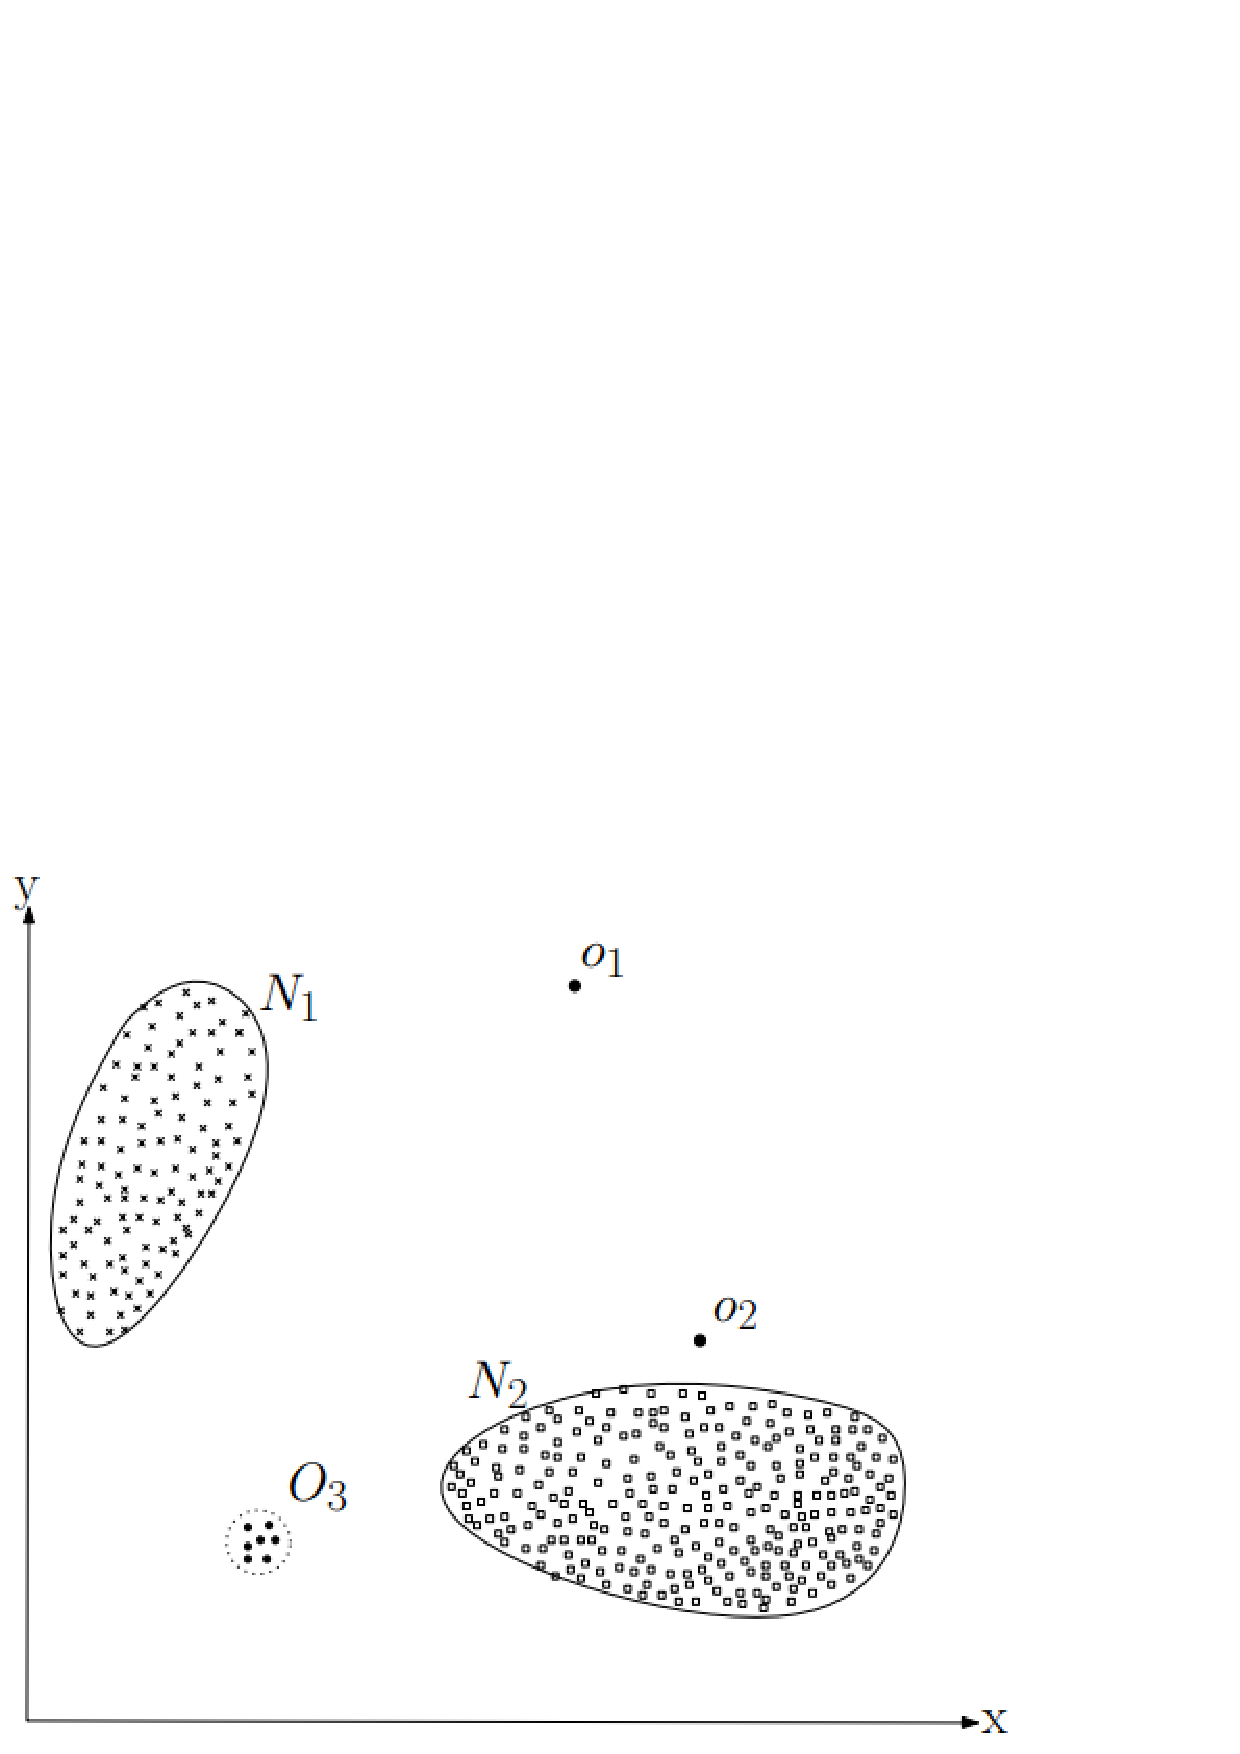
\includegraphics[width=0.5\textwidth]{2d-anomalies.png}
\else
	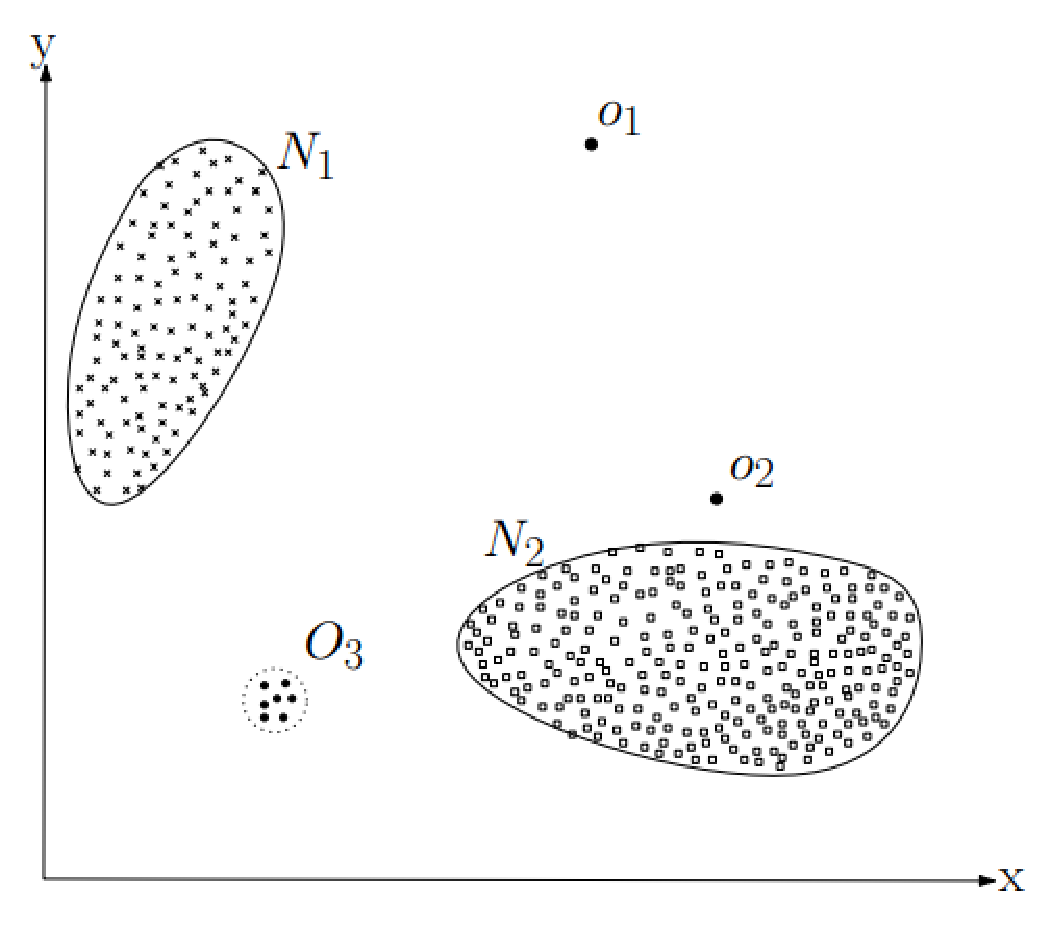
\includegraphics[width=0.5\textwidth]{2d-anomalies.eps}
\fi
\caption{A simple example of anomalies in a 2-dimensional data set.}
\label{fig:2d-anomalies}
\end{figure}

% CHALLENGES
\subsection{Challenges}
\label{sec:anomalyDetection:challenges}
At an abstract level, an anomaly is defined as a pattern that does not conform 
to expected normal behavior \cite{Chandola:2007}. A straightforward anomaly 
detection approach, therefore, is to define a region representing normal 
behaviour and declare any observation in the data which does not belong to this 
normal region as an anomaly. But several factors make this apparently simple 
approach very challenging:

\begin{itemize}
\item Defining a normal region which encompasses every possible normal behaviour 
is very difficult. In addition, the boundary between normal and anomalous 
behaviour is often not precise. Thus an anomalous observation which lies close
to the boundary can actually be normal, and vice-versa.
\item When anomalies are the result of malicious actions, the malicious 
adversaries often adapt themselves to make the anomalous observations appear 
like normal, thereby making the task of defining normal behavior more difficult.
\item In many domains normal behavior keeps evolving and a current notion of
normal behavior might not be su±ciently representative in the future.
\item The exact notion of an anomaly is different for different application 
domains. For example, in the medical domain a small deviation from normal (for
example, fluctuations in body temperature) might be an anomaly, while similar 
deviation in the stock market domain (for example, fluctuations in the value of 
a stock) might be considered as normal. Thus applying a technique developed in 
one domain to another is not straightforward.
\item Availability of labeled data for training/validation of models used by 
anomaly detection techniques is usually a major issue.
\item Often the data contains noise which tends to be similar to the actual 
anomalies and hence is di±cult to distinguish and remove.
\end{itemize}

Due to the above challenges, the anomaly detection problem, in its most general
form, is not easy to solve. In fact, most of the existing anomaly detection 
techniques solve a specific formulation of the problem. The formulation is 
induced by various factors such as nature of the data, availability of labeled 
data, type of anomalies to be detected, etc. Often, these factors are determined
by the application domain in which the anomalies need to be detected. 
Researchers have adopted concepts from diverse disciplines such as statistics, 
machine learning, data mining, information theory, spectral theory, and have 
applied them to specific problem formulations.

\subsection{Types of anomalies}
\label{sec:typesOfAnomalies}
Anomalies can be classified into three categories \cite{Chandola:2007}:

\begin{description}
\item[Point anomaly] If an individual data instance can be considered as 
anomalous with respect to the rest of data, then the instance is termed as a 
point anomaly. This is the simplest type of anomaly. Referring to 
\hyperref[fig:2d-anomalies]{Figure~\ref{fig:2d-anomalies}}, points $o_{1}$ and 
$o_{2}$, as well as all points in region $O_{3}$ lie outside the boundary of the
normal regions, and are hence point anomalies.

\item[Contextual anomalies] If a data instance is anomalous in a certain 
context, but not otherwise, then it is termed a contextual anomaly. The notion 
of a context is induced by the structure in the data set and has to be specified
as part of the problem formulation.

\begin{figure}
\centering
\ifpdf
	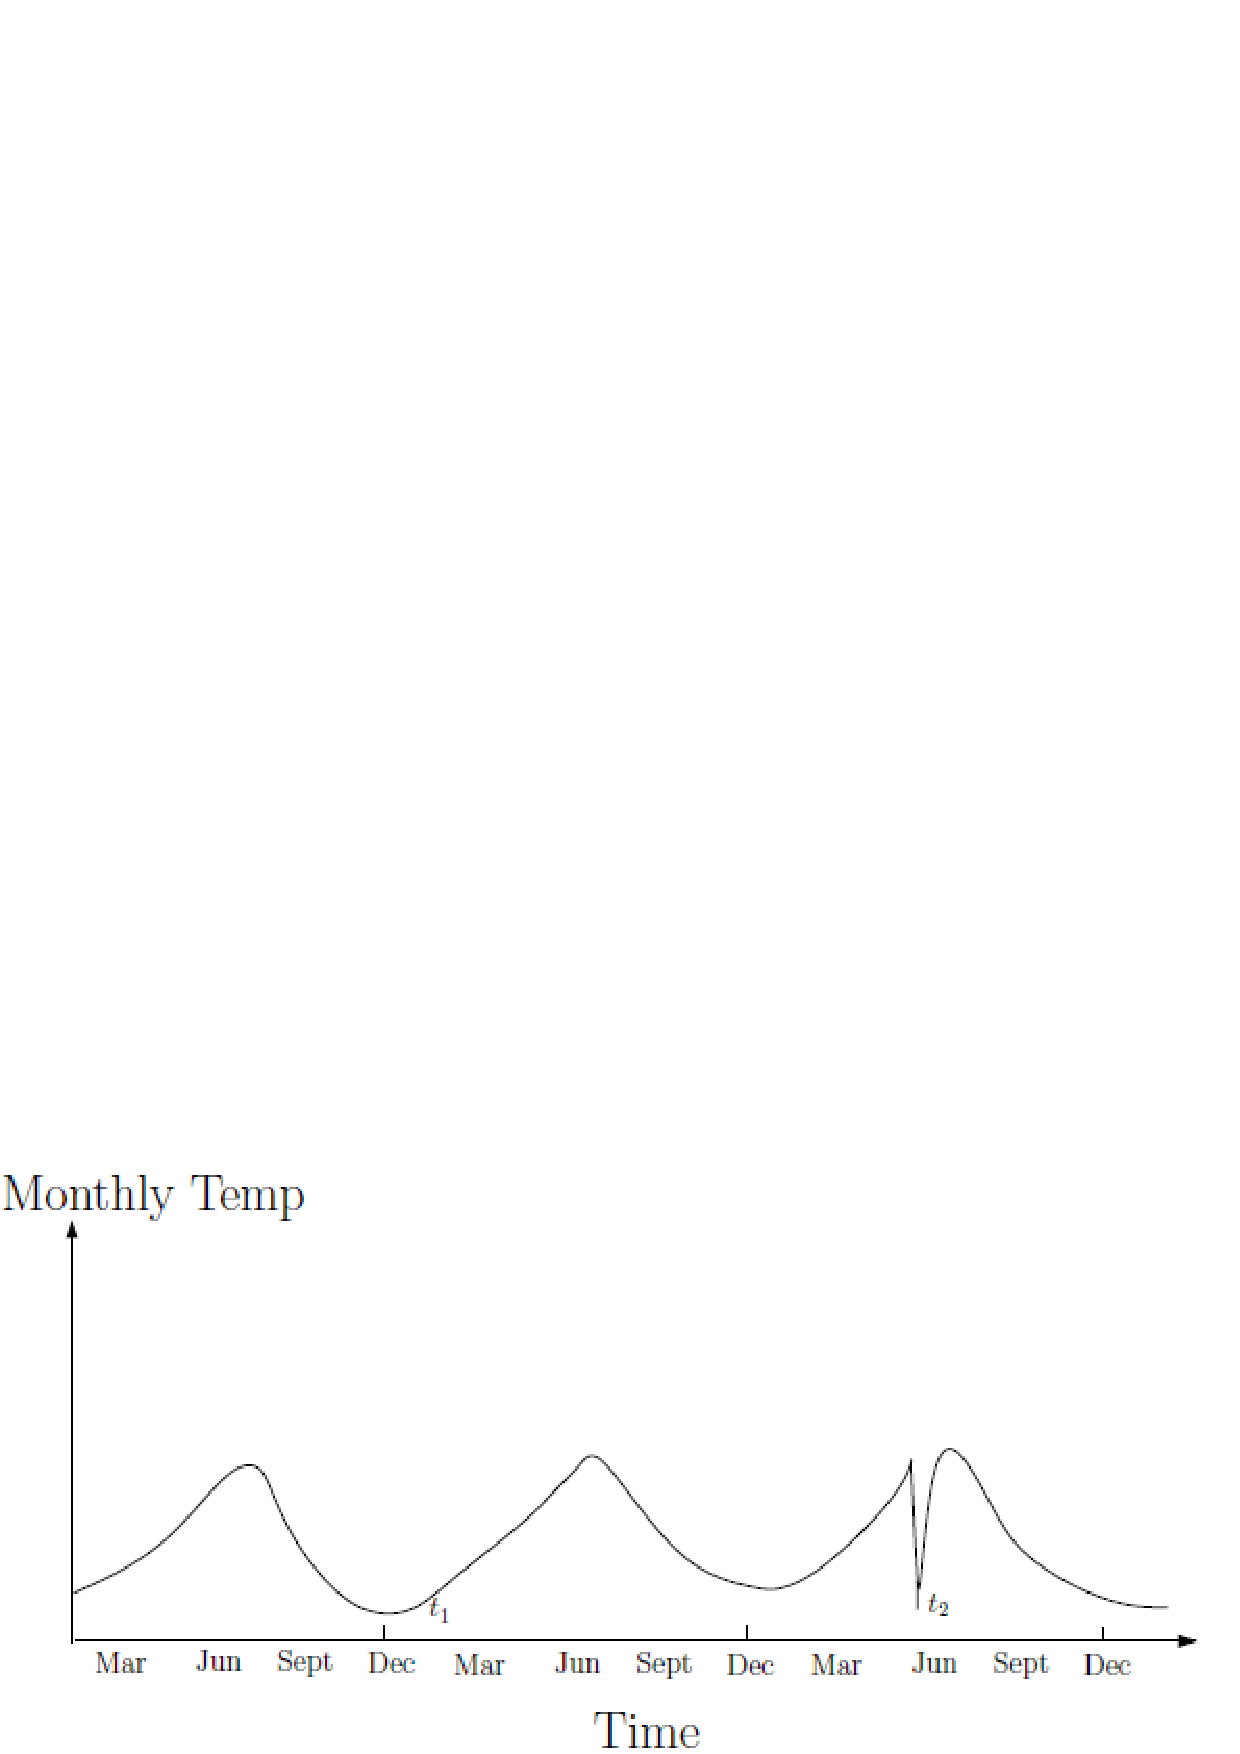
\includegraphics[width=0.5\textwidth]{contextual-anomalies.png}
\else
	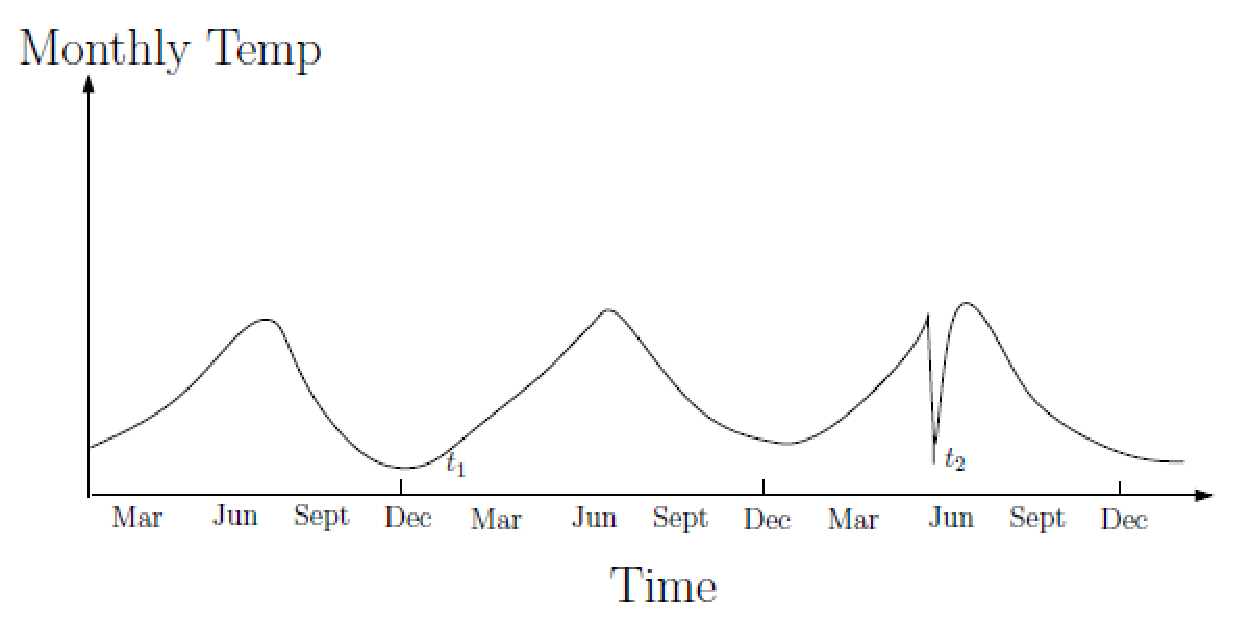
\includegraphics[width=0.5\textwidth]{contextual-anomalies.eps}
\fi
\caption{Contextual anomaly $t_{2}$ in a temperature time series. Note that the 
temperature at time $t_{1}$ is same as that at time $t_{2}$ but occurs in a 
different context and hence is not considered as an anomaly.}
\label{fig:contextual-anomalies}
\end{figure}

Contextual anomalies have been most commonly explored in time-series data and 
spatial data. \hyperref[fig:contextual-anomalies]
{Figure~\ref{fig:contextual-anomalies}} shows one such example for a temperature
time series which shows the monthly temperature of an area over last few years. 
A temperature of 35F might be normal during the winter (at time $t_{1}$) at that
place, but the same value during summer (at time $t_{2}$) would be an anomaly.

\item[Collective anomalies] If a collection of related data instances is 
anomalous with respect to the entire data set, it is termed as a collective 
anomaly. The individual data instances in a collective anomaly may not be 
anomalies by themselves, but their occurrence together as a collection is 
anomalous. \hyperref[fig:collective-anomalies]
{Figure~\ref{fig:collective-anomalies}} illustrates an example which shows a 
human electrocardiogram output \cite{Goldberger:2000}. The highlighted region 
denotes an anomaly because the same low value exists for an abnormally long 
time. Note that that low value by itself is not an anomaly.

\begin{figure}
\centering
\ifpdf
	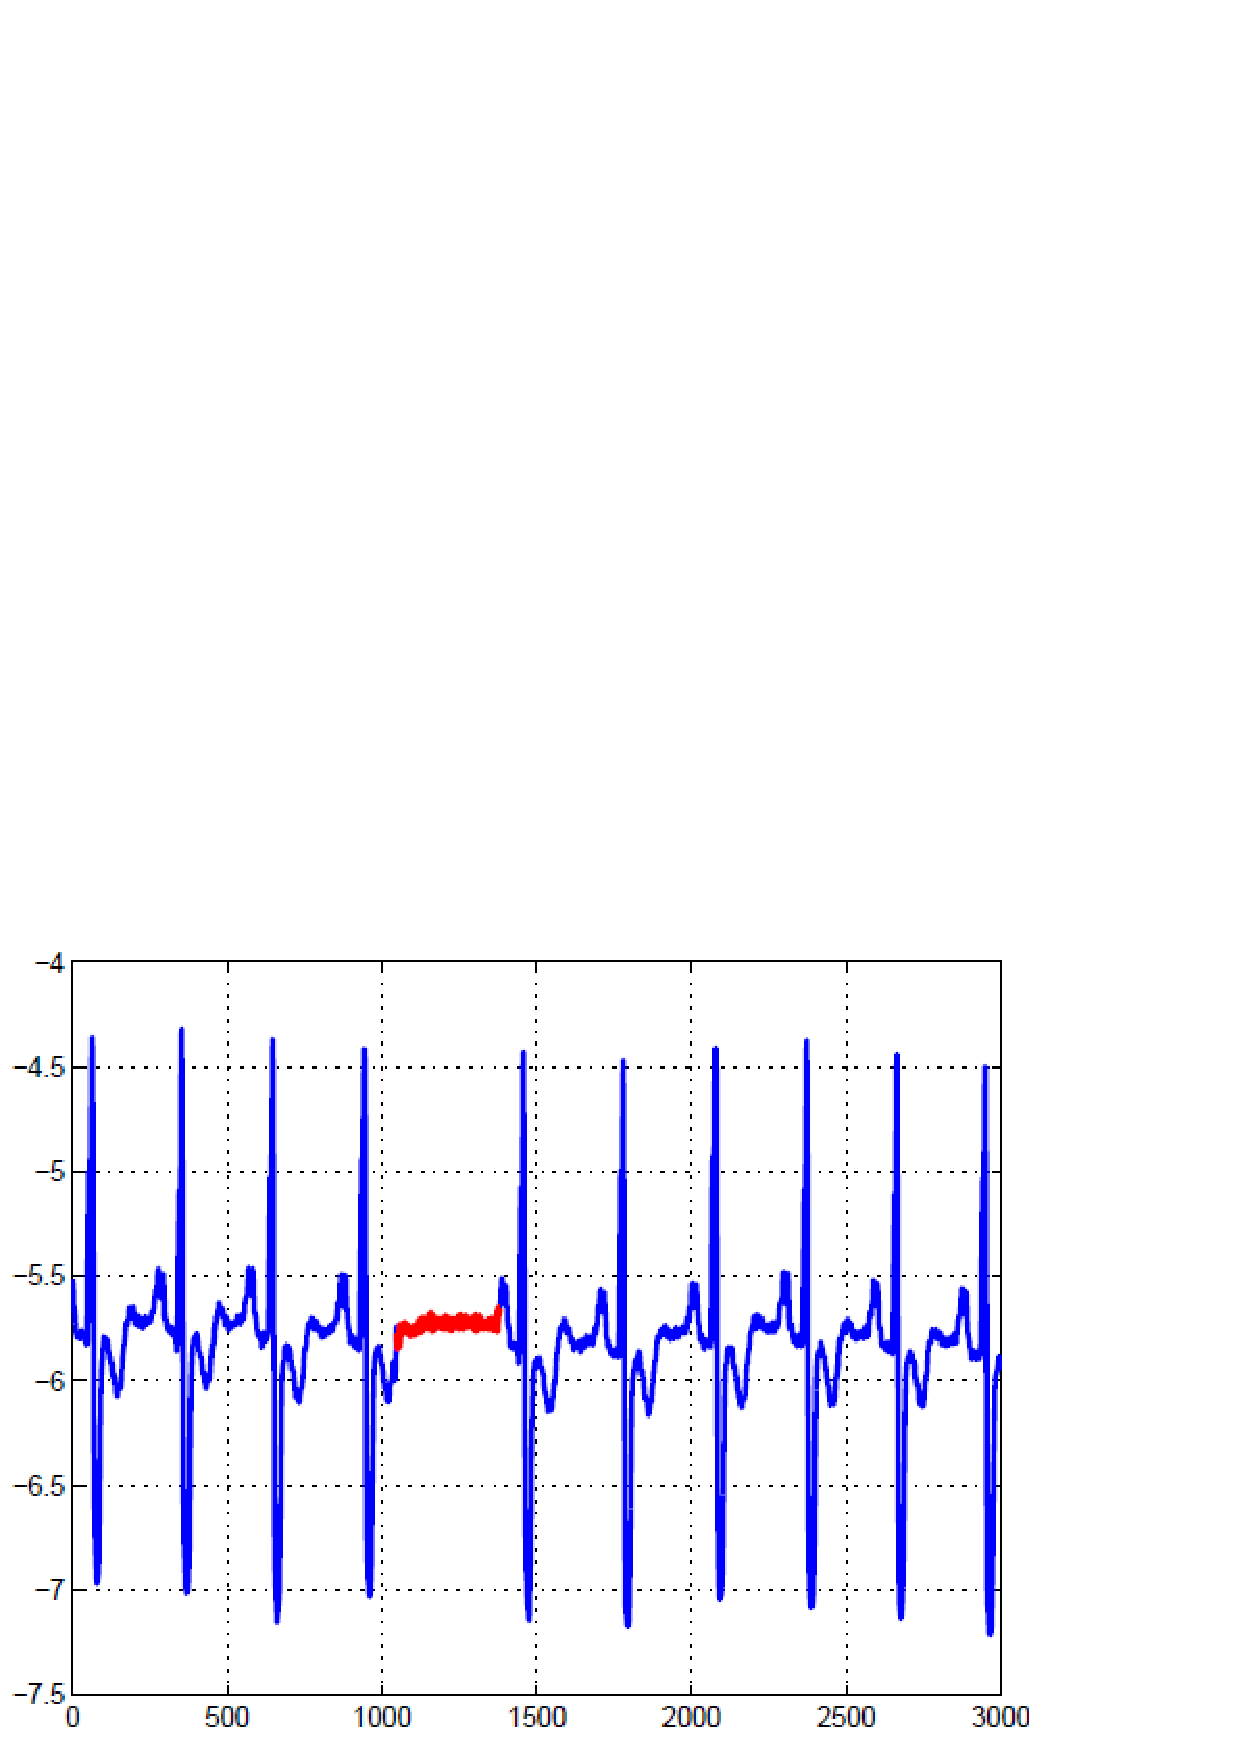
\includegraphics[width=0.5\textwidth]{collective-anomalies.png}
\else
	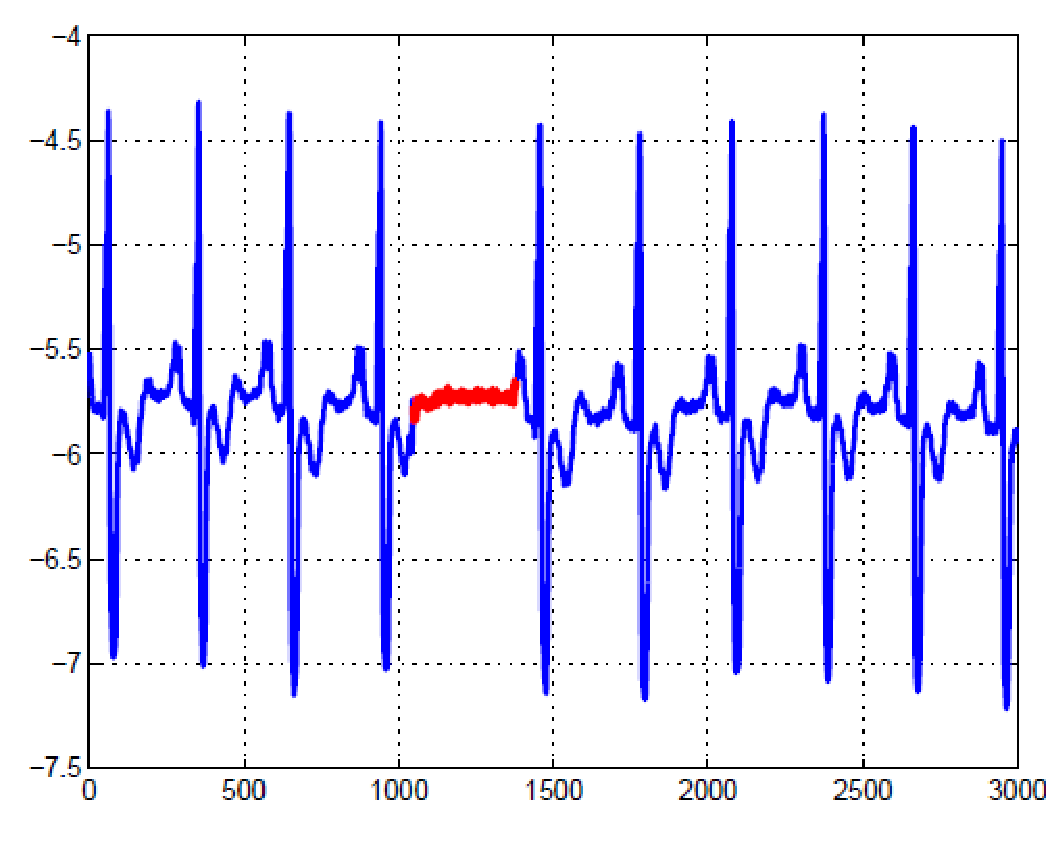
\includegraphics[width=0.5\textwidth]{collective-anomalies.eps}
\fi
\caption{TODO}
\label{fig:collective-anomalies}
\end{figure}

\end{description}

% APPROACHES
\subsection{Approaches}
Traditional approaches to anomaly detection use statistical easures to judge 
data points as outliers. Statistical methods are often model-based and assume 
that the data should follow some distribution. With knowledge of the 
distribution, data point are evaluated by their fitness to the assumed 
distribution. If the probibility of a data instance is less than a certain 
threshold, then that data point is considered an anomaly.

A common distribution considered when modelling data is the `Normal' 
distribution. The probability that a data instance lies within $k$ standard 
deviations $\sigma$ from the mean $\mu$ is the area between $\mu - k\sigma$ and 
$\mu + k\sigma$.

%%%%%%%%%%%%%%%%%%%%%%%%%%%%%%%%%%%%%%%%%%%%%%%%%
% OUTLIERS
%%%%%%%%%%%%%%%%%%%%%%%%%%%%%%%%%%%%%%%%%%%%%%%%%
\section{Outliers}
\label{sec:outliers}
A similar concept to that of anomalies is the concept of outlier. The terms 
``anomaly'' and ``outlier'' are almost used synonymously, but do vary slightly 
in their definition.

In general, two different kinds of outliers exist: global outliers and local 
outliers. Global outliers are distinct with respect to the whole data set, while
local outliers are distinct with respect to data points in their local 
neighbourhood \cite{Vries:2011}. The task of global outlier detection has 
undergone much research, but this has not been the case for local outlier 
detection. In their paper ``Density-preserving projections for large-scale local
anomaly detection'', De Vries et al optimise the use of local outlier factor 
(LOF) for large and high-dimensional data and propose projection-indexed 
nearest-neighbours (PINN) --- a novel technique that exploits extended 
nearest-neighbour sets in a reduced-dimensional space to create an accurate 
approximation for k-nearest-neighbour distances, which is used as the core 
density measurement within LOF \cite{Vries:2011}.

\subsection{Local Outlier Factor}
\label{sec:localOutlierFactor}
`Local Outlier Factor' is a formula that captures the degree to which a data 
point is an outlier with respect to its local neighbourhood. In this context,
`local' means that the determination of the data points does not depend on 
knowledge of the global distribution of the data set.

\subsection{Outlier detection}
\label{sec:outlierDetection}
In this section we will review some general definitions which may be used to 
classify local outliers.

\begin{description}

\item[Classical] A point is declared to be an outlier if its distance from the 
mean is sufficiently large.
\item[Principal Component Analysis] An outlier is usually declared if the point 
is sufficiently far away from the subspace spanned by the eigenvectors 
corresponding to the highest eigenvalues.
\item[Distance based] A point can be declared to be an outlier if its distance 
to its kth nearest-neighbour is sufficiently large.

\end{description}

%%%%%%%%%%%%%%%%%%%%%%%%%%%%%%%%%%%%%%%%%%%%%%%%%
% RANDOM PROJECTIONS
%%%%%%%%%%%%%%%%%%%%%%%%%%%%%%%%%%%%%%%%%%%%%%%%%
\section{Random projections}
\label{sec:randomProjections}
% TODO

%%%%%%%%%%%%%%%%%%%%%%%%%%%%%%%%%%%%%%%%%%%%%%%%%
% MARKOV CHAINS
%%%%%%%%%%%%%%%%%%%%%%%%%%%%%%%%%%%%%%%%%%%%%%%%%
\section{Markov chains}
\label{sec:markovChains}
A `Markov chain' is a chance process in which the outcome of a given experiment 
can affect the outcome of the next experiment \cite{Grinstead:1997}. For a 
Markov chain, we have a set of states $S = \left\{ s_{1}, s_{2}, \ldots, s_{r} 
\right\}$ with a process starting in one of the states and moving from state 
$s_{i}$ to $s_{j}$ with a probability $p_{ij}$ not dependent upon which states 
the chain was in before the current state. The probabilities $p_{ij}$ are called
\emph{transition probabilities}, and the complete matrix $\mathbf{P}$ of 
probabilities is known as the \emph{transition matrix}.

The probability that, given the chain is in state $i$ now, it will be in state 
$j$ in two steps is denoted by $p_{ij}^{(2)}$. In general, if a Markov chain has 
$r$ states, then:

\begin{displaymath}
p_{ij}^{(2)} = \sum_{k=1}^{r} p_{ik}p{kj}
\end{displaymath}

%%%%%%%%%%%%%%%%%%%%%%%%%%%%%%%%%%%%%%%%%%%%%%%%%
% RANDOM WALKS ON GRAPHS
%%%%%%%%%%%%%%%%%%%%%%%%%%%%%%%%%%%%%%%%%%%%%%%%%
\section{Random walks on graphs}
\label{sec:randomWalks}

Assume we are given a connected undirected and weighted graph $G = (V,E,W)$ with
edge weights $(w_{ij})_{i,j \in V} >= 0$ be the graph adjacency matrix. A degree
of a node $i$ is $d_{i} = \sum_{j \in N(i)} w_{ij}$ where $N(i)$ is a set of 
neighbours of node $i$. All nodes nonadjacent to $i$ are assumed to have a 
weight of $w_{ij} = 0$.

A random walk is a sequence of nodes on a graph visited by a random walkter: 
starting from a node, the random walker moves to one of its neighbours with some
probability. Then from that node, it proceeds to one of its own neighbours with 
some probability, and so on \cite{Khoa:2012}. The random walk is a finite Markov
chain that is time-reversible, which means the reverse Markov chain has the same
transition probability matrix as the original Markov chain \cite{Lovasz:1996}.

The probability that a random walker selects a particular node from is 
neighbours is determined by the edge weights of the graph. The larger the weight
${w_ij}$ of the edge connecting nodes $i$ and $j$, the more often the random 
walker travels through that edge.

%%%%%%%%%%%%%%%%%%%%%%%%%%%%%%%%%%%%%%%%%%%%%%%%%
% DISTANCE METRICS
%%%%%%%%%%%%%%%%%%%%%%%%%%%%%%%%%%%%%%%%%%%%%%%%%
\section{Distance metrics}
\label{sec:distanceMetrics}
Distance is a quantitative description of how far apart two objects are. 
Mathematically, a distance or metric is a function describing how close or far 
away data points in some space are from each other \cite{Khoa:2012}.

% EUCLIDEAN DISTANCE
\subsection{Euclidean distance}
\label{sec:euclideanDistance}
An Euclidean distance between two data points in a space is the norm of the 
difference between two vectors corresponding to these data points 
\cite{Khoa:2012}. Euclidean distance is extremely sensitive to the scale of the 
features involved. When dealing with features of vastly different scales, the 
effects of the larger feature dominant over the smaller feature in terms of the 
Euclidean distance. This problem is usually solved by normalizing the data 
values. Another issue, however, with Euclidean distance is that it is unable to 
take into account any correlation between data features.

% MAHALANOBIS DISTANCE
\subsection{Mahalanobis distance}
\label{sec:mahalanobisDistance}
Mahalanobis distance is a distance measure that considers the covariance between
data features. Mahalanobis distance, however, is extremely sensitive to 
anomalies as anomalies affect both the mean and the covariance of the data.

% GRAPH GEODESIC DISTANCE
\subsection{Graph geodesic distance}
\label{sec:graphGeodesicDistance}

%%%%%%%%%%%%%%%%%%%%%%%%%%%%%%%%%%%%%%%%%%%%%%%%%
% NEAREST NEIGHBOUR ALGORITHMS
%%%%%%%%%%%%%%%%%%%%%%%%%%%%%%%%%%%%%%%%%%%%%%%%%
\section{Nearest Neighbour Algorithms}
\label{sec:nearestNeighbourAlgorithms}

%%%%%%%%%%%%%%%%%%%%%%%%%%%%%%%%%%%%%%%%%%%%%%%%%
% VECTORS AND MATRICES
%%%%%%%%%%%%%%%%%%%%%%%%%%%%%%%%%%%%%%%%%%%%%%%%%
\section{Vectors and Matrices}
\label{sec:vectorsAndMatrices}

% EIGENVECTORS AND EIGENVALUES
\subsection{Eigenvectors and Eigenvalues}
\label{sec:eigenvectorsAndEigenvalues}
This section will briefly recall some basic definitions of eigenvectors and
eigenvalues, as well as some of their basic properties.

A vector $\mathbf{v}$ is an eigenvector of a matrix $M$ of eigenvalue $\lambda$ 
if:
\begin{displaymath}
M\mathbf{v} = \lambda\textbf{v}
\end{displaymath}

If $\mathbf{v_{1}}$ is an eigenvector of M of eigenvalue $\lambda_{1}$, 
$\mathbf{v_{2}}$ is an eigenvector of M of eigenvalue $\lambda_{2} \neq 
\lambda_{1}$, and $M$ is symmetric, then $\mathbf{v_{1}}$ is orthogonal to 
$\mathbf{v_{2}}$.

For a symmetric matrix $M$, the multiplicity of an eigenvalue $\lambda$ is the
dimension of the space of eigenvectors of eigenvalue $\lambda$. Also recall that
every $n{\times}n$ symmetric matrix has $n$ eigenvalues, counted with 
multiplicity. Thus, it has an orthonormal basis of eigenvectors, 
$\begin{Bmatrix} \mathbf{v_{1}} & \ldots & \mathbf{v_{n}} \end{Bmatrix}$ with
eigenvalues $\lambda_{1} \leq \lambda_{2} \leq \ldots \leq \lambda_{n}$ so that:
\begin{displaymath}
M\mathbf{v_{i}} = \lambda_{i}\mathbf{v_{i}} \quad \forall i
\end{displaymath}

If we let $V$ be the matrix whose $i$th column is $v_{i}$ and $\Lambda$ be the 
diagonal matrix whose $i$th diagonal is $\lambda_{i}$, we can write this more 
compactly as:
\begin{displaymath}
MV = V\Lambda
\end{displaymath}

Multiplying by $V^{T}$ on the right, we obtain the eigen-decompisition of $M$:
\begin{displaymath}
M = MVV^{T} = V{\Lambda}V^{T} = \sum_{i} \lambda_{i}\mathbf{v_{i}}\mathbf{v_{i}^{T}}
\end{displaymath}

% EIGEN DECOMPOSITION
\subsection{Eigen decomposition}
\label{sec:eigenDecomposition}

% LAPLACIAN MATRICES
\subsection{Laplacian Matrices}
\label{sec:laplacianMatrices}
\nocite{Berkeley:1999}
\nocite{Pati:2011}
\nocite{Spielman:2006}
Recall that a weighted, undirected graph $G = (V,E,w)$ is essentially an 
undirected graph $G = (V,E)$ along with a function $w : E \rightarrow 
\Re^{+}$, where $\Re^{+}$ denotes the set of positive real numbers.

The adjacency matrix of a weighted graph $G$ will be denoted $A_{G}$, and is
given by:
\begin{displaymath}
A_{G}(i,j) := 
    \left\{
        \begin{array}{ll}
            \mathit{w}(i,j) &   \quad \text{if $(i,j) \in E$} \\
            0 &                 \quad \text{otherwise}
        \end{array}
    \right.
\end{displaymath}

The degree matrix of a weighted graph $G$ will be denoted $D_{G}$, and is the
diagonal matrix such that:
\begin{displaymath}
D_{G}(i,i) = \sum_{j} A_{G}(i,j)
\end{displaymath}

A Laplacian Matrix is a matrix representation of a graph, defined by the
equation:
\begin{displaymath}
L_{G} = D_{G} - A_{G}
\end{displaymath}

Now, let $G_{1,2}$ be a graph on two vertices with a single edge of weight $1$.
\begin{displaymath}
L_{G_{1,2}} :=
    \begin{bmatrix}
        1 & -1 \\
        -1 & 1
    \end{bmatrix}
\end{displaymath}

For the graph with $n$ vertices and just one edge between vertices $u$ and $v$, 
we can define the Laplacian Matrix similarly. For concreteness, I'll call this
graph $G_{u,v}$. It's Laplacian Matrix is the $n{\times}n$ matrix whose only 
non-zero entries are in the intersections of rows and columns $u$ and $v$. The 
$2{\times}2$ matrix at the intersections of these rows and columns is, of 
course:
\begin{displaymath}
    \begin{bmatrix}
        1 & -1 \\
        -1 & 1
    \end{bmatrix}
\end{displaymath}

For a weighted graph $G = (V,E,w)$, we define:
\begin{displaymath}
L_{G} := \sum_{(u,v) \in E} w(u,v)L_{G_{u,v}}
\end{displaymath}

\paragraph{Properties}
For a graph $G$ and its Laplacian Matrix $L$ with eigenvalues $\lambda_{0} < 
\lambda_{1} < \ldots < \lambda_{n-1}$:

\begin{itemize}
\item $L$ is a symmetric matrix. This means the eigenvalues of $L$ are real, and
its eigenvectors are real and orthogonal.
\item $L$ is always positive-semidefinite ($\forall i, \lambda_{i} \geq 0; 
\lambda_{0} = 0$).
\item Let $G = (V,E)$ be a graph, and let $0 = \lambda_{1} \leq \lambda_{2}
\leq \ldots \leq \lambda_{n}$ be the eigenvalues of its Laplacian Matrix. Then, 
$\lambda_{2} > 0$ if and only if $G$ is connected.
\item The number of times $0$ appears as an eigenvalue in the Laplacian Matrix 
is the number of connected components in the graph.
\item $\lambda_{0}$ is always $0$ because every Laplacian Matrix has an 
eigenvector of $\begin{bmatrix} 1 & 1 & \ldots & 1 \end{bmatrix}$ that, for each
row, adds the corresponding node's degree to a ``-1'' for each neighbour, 
thereby producing zero by definition.
\item The smallest non-zero eigenvalue of $L$ is called the spectral gap.
\item If we arbitarily assign an orientation to the edges in $G$ and label each
edge, then we can define the vertex edge incidence matrix $Q$ by:
\begin{displaymath}
Q_{ij} := 
    \left\{
        \begin{array}{ll}
            1 &     \quad \text{if $e_{j}$ starts from $i$} \\
            -1 &    \quad \text{if $e_{j}$ ends at $i$} \\
            0 &     \quad \text{otherwise}
        \end{array}
    \right.
\end{displaymath}
Then the Laplacian Matrix $L$ satisfies $L = Q^{T}Q$, regardless of the 
orientation of the edges.
\item The second smallest eigenvalue of $L$ ($\lambda_{2}$) is the algebraic 
connectivity of $G$. $\lambda_{2} > 0$ if and only if $G$ is connected.
\end{itemize}

%%%%%%%%%%%%%%%%%%%%%%%%%%%%%%%%%%%%%%%%%%%%%%%%%
% COMMUTE TIME
%%%%%%%%%%%%%%%%%%%%%%%%%%%%%%%%%%%%%%%%%%%%%%%%%
\section{Commute Time}
\label{sec:commuteTime}

% INTRODUCTION
\subsection{Introduction}
\label{sec:commuteTime:introduction}
Commute time is a robust distance metric derived from a random walk on graphs 
\cite{Khoa:2012}. In his thesis on ``Large Scale Anomaly Detection and 
Clustering Using Random Walks'', Khoa demonstrated how commute time can be used 
as a distance measure for data mining tasks such as anomaly detection and 
clustering. A prohibitive limitation of this techniue is that the calculation of
commute time involves the eigen decomposition of the graph Laplacian, making it 
impractical for large graphs.

A major advantage of using commute time as a distance metric for outlier 
detection is that it effectively captures not only the distances between data 
points but also the density of the data. This property results in a distance 
metric that can be effectively used to capture global, local and group 
anomalies.

The commute time between two nodes $i$ and $j$ in a graph is the number of steps
that a random walk, starting from $i$ will take to visit $j$ and then come back 
to $i$ for the first time. The fact that the commute time is averaged over all 
paths (and not justthe shortest path) makes it more robust to data perturbations
and it can also capture graph density \cite{Khoa:2012}. Since it is a measure 
which can capture the geometrical structure of the data and is robust to noise, 
commute time can be applied in methods where Euclidean or other distances are 
used and thus the limitations of these metrics can be avoided.

% LIMITATIONS
\subsection{Limitations}
\label{sec:commuteTime:limitations}
The computation of commute time requires the eigen decomposition (see 
\hyperref[sec:eigenDecomposition] {Section~\ref{sec:eigenDecomposition}}) of the
graph Laplacianmatrix (see \hyperref[sec:laplacianMatrices] 
{Section~\ref{sec:laplacianMatrices}}), a computation which takes $O(n^{3})$ 
time and thus is not practical for large graphs. Methods to approximate the 
commute time to reduce the computational time are required in order to 
efficiently use commute time in large datasets.

% ANOMALY DETECTION USING COMMUTE TIME
\subsection{Anomaly Detection Using Commute Time}
\label{sec:anomalyDetectionUsingCommuteTime}

\begin{algorithmic}
\If {$i\geq maxval$}
    \State $i\gets 0$
\Else
    \If {$i+k\leq maxval$}
        \State $i\gets i+k$
    \EndIf
\EndIf
\end{algorithmic}

%%%%%%%%%%%%%%%%%%%%%%%%%%%%%%%%%%%%%%%%%%%%%%%%%
% SOLVERS
%%%%%%%%%%%%%%%%%%%%%%%%%%%%%%%%%%%%%%%%%%%%%%%%%
\section{Solvers}
\label{sec:solvers}

% SPIELMAN-TENG SOLVER
\subsection{Spielman-Teng Solver}
\label{sec:spielmanTengSolver}
\nocite{Spielman:2006}
Spielman and Teng presented a randomised algorithm that, on input a symmetric, 
weakly diagonally dominant $n{\times}x$ matrix $A$ with $m$ non-zero entries and
an $n$-vector $\mathbf{b}$, produces an $\tilde{\mathbf{x}}$ such that 
$\begin{Vmatrix} \tilde{\textbf{x}} - A^{\dagger}\textbf{b} \end{Vmatrix}_{A} 
\leq \epsilon \begin{Vmatrix} A^{\dagger}\mathbf{b} \end{Vmatrix}_{A}$ in 
expected time:
\begin{displaymath}
m \log^{O(1)} n \log (1/\epsilon)
\end{displaymath}


%%%%%%%%%%%%%%%%%%%%%%%%%%%%%%%%%%%%%%%%%%%%%%%%%
% CHAPTER 03: Reconfigurable Computing
%%%%%%%%%%%%%%%%%%%%%%%%%%%%%%%%%%%%%%%%%%%%%%%%%
\chapter{Reconfigurable Computing}
\label{ch:reconfigurableComputing}

%%%%%%%%%%%%%%%%%%%%%%%%%%%%%%%%%%%%%%%%%%%%%%%%%
% Introduction
%%%%%%%%%%%%%%%%%%%%%%%%%%%%%%%%%%%%%%%%%%%%%%%%%
\section{Introduction}
\label{sec:rcIntroduction}
\input{ch03-introduction}

%%%%%%%%%%%%%%%%%%%%%%%%%%%%%%%%%%%%%%%%%%%%%%%%%
% Field-Programmable Gate Array (FPGA)
%%%%%%%%%%%%%%%%%%%%%%%%%%%%%%%%%%%%%%%%%%%%%%%%%
\section{Field-Programmable Gate Array (FPGA)}
\label{sec:FPGA}
\input{ch03-fpga}

%%%%%%%%%%%%%%%%%%%%%%%%%%%%%%%%%%%%%%%%%%%%%%%%%
% Application-Specific Integrated Circuit (ASIC)
%%%%%%%%%%%%%%%%%%%%%%%%%%%%%%%%%%%%%%%%%%%%%%%%%
\section{Application-Specific Integrated Circuit (ASIC)}
\label{sec:ASIC}
\input{ch03-asic}

%%%%%%%%%%%%%%%%%%%%%%%%%%%%%%%%%%%%%%%%%%%%%%%%%
% Hardware Description Languages
%%%%%%%%%%%%%%%%%%%%%%%%%%%%%%%%%%%%%%%%%%%%%%%%%
\section{Hardware Description Languages}
\label{sec:HDL}
% VHSIC Hardware Description Language (VHDL)
\subsection{VHSIC Hardware Description Language (VHDL)}

% Verilog (IEEE 1364)
\subsection{Verilog (IEEE 1364)}

% High-Level Synthesis
\subsection{High-Level Synthesis}



%%%%%%%%%%%%%%%%%%%%%%%%%%%%%%%%%%%%%%%%%%%%%%%%%
% CHAPTER 04: Design
%%%%%%%%%%%%%%%%%%%%%%%%%%%%%%%%%%%%%%%%%%%%%%%%%
\chapter{Design}
\label{ch:design}

\section{Introduction}
\label{sec:designIntroduction}

% ALGORITHM PROFILING
\section{Algorithm Profiling}
\label{sec:algorithmProfiling}
In order to choose which step of the algorithm would be best suited for 
implementation on FPGA hardware, it was first necessary to first profile the 
execution of the algorithm using various test cases. This task was performed 
using MATLAB, using code supplied by \citeauthor{Khoa:2012} that was used to 
test and verify the conclusions of \citetitle{Khoa:2012}. Using \emph{MATLAB}'s 
\verb+profile+ command, I was able to analyse the algorithm and make an 
assessment of the running time of the algorithm. The results of the algorithm 
profiling can be found in 
\hyperref[apdx:algorithmProfiling]{Appendix~\ref{apdx:algorithmProfiling}}. 

% PERFORMANCE BOTTLENECK
\subsection{Performance Bottleneck}
\label{sec:algorithmPerformanceBottleneck}
From observations of the results of the algorithm profiling, it was observed 
that the performance of the `anomaly detection using commute-distance' 
algorithm is bottlenecked significantly by a function named 
\verb+TopN_Outlier_Pruning_Block+. The MATLAB code for this function can be 
found in \hyperref[apdx:matlabCode]{Appendix~\ref{apdx:matlabCode}}. Analysis of
this function, as well as discussions with \citeauthor{Khoa:2012} revealed that
the algorithm was originally devised by \citeauthor{Bay:2003} and published in
the paper \citetitle{Bay:2003}. The general steps of the algorithm are described
in \hyperref[algm:TopNOutlierPruningBlock]
{Algorithm~\ref{algm:TopNOutlierPruningBlock}}.

\begin{algorithm}[t]
\caption{TopN\_Outlier\_Pruning\_Block}
\label{algm:TopNOutlierPruningBlock}

\LinesNumbered

\SetKwInput{InputK}{k}
\SetKwInput{InputN}{N}
\SetKwInput{InputD}{Data}
\SetKwInOut{OutputO}{outliers}

\InputK{the number of nearest neighbors}
\InputN{the number of outliers to return}
\InputD{a set of examples in random order}
\OutputO{a set of outliers}

\SetKwData{varB}{b}
\SetKwData{Block}{block}
\SetKwData{Cutoff}{cutoff}
\SetKwData{varD}{d}
\SetKwData{Data}{Data}
\SetKwData{varK}{k}
\SetKwData{varN}{N}
\SetKwData{Neighbours}{neighbours}
\SetKwData{varO}{o}
\SetKwData{Outliers}{outliers}
\SetKwData{Score}{score}

\SetKwFunction{Closest}{closest}
\SetKwFunction{Distance}{distance}
\SetKwFunction{GetNextBlock}{getNextBlock}
\SetKwFunction{MaxDist}{maxDist}
\SetKwFunction{Min}{min}
\SetKwFunction{Top}{top}

\Begin{
	$\Cutoff \longleftarrow 0$\tcp*[l]{set the cutoff for pruning to $0$}
	$\Outliers \longleftarrow \emptyset$\tcp*[l]{initialize to the empty set}
	\BlankLine
	\While(\tcp*[h]{load a block of examples from \varD}){$\Block \longleftarrow \GetNextBlock{\Data}$}{
		$\Neighbours(\varB) \longleftarrow \emptyset, \quad \forall \, \varB \in \Block$\;
		\BlankLine
		\ForEach{$\varD \in \Data$}{
			\ForEach{$\varB \in \Block \: : \: \varB \neq \varD$}{
				\If{$|\Neighbours(\varB)| < \varK \: \lor \: \Distance{\varB, \varD} < \MaxDist{\varB, \Neighbours(\varB)}$}{
					$\Neighbours(\varB) \longleftarrow \Closest{\varB, \Neighbours(\varB)} \cup \varD, \varK)$\;
					\If{$\Score(\Neighbours(\varB), \varB) < \Cutoff$}{
						$\Block \longleftarrow \Block \setminus \varB$\;
					}
				}
			}
		}
		\BlankLine
		$\Outliers \longleftarrow $\Top{$\Block \cup \Outliers$, $\varN$}\tcp*[l]{keep only the top n outliers}
		$\Cutoff \longleftarrow \Min_{\varO \in \Outliers}(\Score(\varO))$\tcp*[l]{the cutoff is the score of the weakest outlier}
	}
	\KwRet{\Outliers}\;
}
\end{algorithm}

In this algorithm, the \verb+score+ function can be any monotonically decreasing
function of the nearest neighbor distances such as the distance to the $k$th 
nearest neighbor, or the average distance to the $k$ neighbours \cite{Bay:2003}.

The main idea of the  nested loop algorithm is that for each example in the 
input set \verb+Data+, the algorithm keeps track of the closest neighbours found
so far. When an example's closest neighbours achieve a score lower than the 
\verb+cutoff+, the example is discarded because it can no longer be an outlier. 
As more examples are processed, the algorithm finds more extreme outliers and 
the \verb+cutoff+ increases along with pruning efficiency \cite{Bay:2003}.

In the worst case, the performance of the algorithm is very poor --- due to the 
nested loops, it could require $O(N^{2})$ distance computations and 
$O(\frac{N}{blocksize} \times N)$ data accesses. However, \citeauthor{Bay:2003} 
proved (through application of the algorithm to both real and synthetic data
sets) that the algorithm performs considerably better than the expected 
$O(N^{2})$ running time in the average case. The performance improvements over 
similar algorithms were attributed to the application of randomization and 
pruning techniques. The outlier pruning problem can be considered similar to the
problem of conducting a set of independent Bernoulli trials in which examples 
are analysed until $k$ examples within distance $d$ are found, or until the data
set is exhausted. \citeauthor{Bay:2003} proved that the number of trials 
expected to achieve $k$ examples within distance $d$ is given by:

\begin{equation}
\label{eqn:outlierPruneComplexity}
E[Y] \leq \frac{k}{\pi(\textbf{x})} + \Bigg(1 - \sum_{y=k}^{N} P(Y=y)\Bigg) \times N
\end{equation}

Where $\pi(x)$ is the probability that a random drawn example lies within 
distance $d$ of point $x$ and $P(Y=y)$ is the probability of obtaining the $k$th 
success on trial $y$.

The first term in \hyperref[eqn:outlierPruneComplexity]
{Equation~\ref{eqn:outlierPruneComplexity}} represents the number of distance 
computations to eliminate non-outliers, and does not depend on $N$. The second 
term represents the expected cost of outliers, and does depend on $N$, yielding 
an overall quadratic dependency to process $N$ examples in total. However, note 
that we typically set the program parameters to return a small and possibly 
fixed number of outliers. Thus the first term dominates and we obtain near 
linear performance \cite{Bay:2003}. More specifically, it was determined that 
the primary factor determining the scaling is how the cutoff changes as $N$ 
increases.

There are, however, some limitations of the aforementioned algorithm. 
Specifically:
\begin{enumerate}
\item The algorithm assumes that the data is in random order. If the data is not
in random order and is sorted then the performance can be poor.
\item The algorithm depends on the independence of examples. If examples are 
dependent in such a way that they have similar values (and will likely be in the
set of $k$ nearest neighbors) this can cause performance to be poor as the
algorithm may have to scan the entire data set to find the dependent examples.
\item The algorithm can perform poorly occurs when the data does not contain 
outliers.
\end{enumerate}


%%%%%%%%%%%%%%%%%%%%%%%%%%%%%%%%%%%%%%%%%%%%%%%%%
% CHAPTER 05: Implementation
%%%%%%%%%%%%%%%%%%%%%%%%%%%%%%%%%%%%%%%%%%%%%%%%%
\chapter{Implementation}
\label{ch:implementation}

%%%%%%%%%%%%%%%%%%%%%%%%%%%%%%%%%%%%%%%%%%%%%%%%%
% CHAPTER 06: Results
%%%%%%%%%%%%%%%%%%%%%%%%%%%%%%%%%%%%%%%%%%%%%%%%%
\chapter{Results}
\label{ch:results}

%%%%%%%%%%%%%%%%%%%%%%%%%%%%%%%%%%%%%%%%%%%%%%%%%
% CHAPTER 07: Conclusions
%%%%%%%%%%%%%%%%%%%%%%%%%%%%%%%%%%%%%%%%%%%%%%%%%
\chapter{Conclusions}
\label{ch:conclusions}

%%%%%%%%%%%%%%%%%%%%%%%%%%%%%%%%%%%%%%%%%%%%%%%%%
% Appendix
%%%%%%%%%%%%%%%%%%%%%%%%%%%%%%%%%%%%%%%%%%%%%%%%%
\appendix

%%%%%%%%%%%%%%%%%%%%%%%%%%%%%%%%%%%%%%%%%%%%%%%%%
% APPENDIX 01: MATLAB code
%%%%%%%%%%%%%%%%%%%%%%%%%%%%%%%%%%%%%%%%%%%%%%%%%
\chapter{MATLAB Code}
\label{apdx:matlabCode}
\input{appendix01}

%%%%%%%%%%%%%%%%%%%%%%%%%%%%%%%%%%%%%%%%%%%%%%%%%
% APPENDIX 02: C code
%%%%%%%%%%%%%%%%%%%%%%%%%%%%%%%%%%%%%%%%%%%%%%%%%
\chapter{C Code}
\label{apdx:cCode}
\input{appendix02}


%%%%%%%%%%%%%%%%%%%%%%%%%%%%%%%%%%%%%%%%%%%%%%%%%
% Bibliography
%%%%%%%%%%%%%%%%%%%%%%%%%%%%%%%%%%%%%%%%%%%%%%%%%
\nocite{*}
\printbibliography

%%%%%%%%%%%%%%%%%%%%%%%%%%%%%%%%%%%%%%%%%%%%%%%%%
% Glossary
%%%%%%%%%%%%%%%%%%%%%%%%%%%%%%%%%%%%%%%%%%%%%%%%%
% \glsaddall
% \printglossary

%%%%%%%%%%%%%%%%%%%%%%%%%%%%%%%%%%%%%%%%%%%%%%%%%
% Index
%%%%%%%%%%%%%%%%%%%%%%%%%%%%%%%%%%%%%%%%%%%%%%%%%
% \printindex

\end{document}
